\section{Nivel 2} \label{Nivel:Niv02}
	\subsection{Título del nivel}
	Nadie cruza mis dominios.
	\subsection{Encuentro}
El nivel le enseñara al jugador las mecánicas de combate: combate simple contra enemigos y el combate contra un jefe. Este nivel estará disponible después de terminar el primer nivel (ver apartado \ref{Nivel:Niv01}).
	\subsection{Descripción}
Malinalli y Xólotl se adentran al inframundo. Su primer reto a superar será cruzar el río de Apanohuaia y sus peligros para poder derrotar al primer guardián del inframundo: la iguana gigante Xochitonal. Xólotl adopta la forma de un ajolote de gran tamaño para que ambos puedan cruzar el río, por lo que el jugador controlara al Sprite de Malinalli sobre un ajolote de gran tamaño. 
	\subsection{Objetivos}
\begin{itemize}
	\item Aprender a utilizar el funcionamiento de los ataques de Malinalli y de los ítems flor de vainilla (ver apartado \ref{item:vainilla}) y grano de cacao (ver apartado \ref{item:cacao}).
	\item El jugador deberá de atravesar el lago derrotando a los enemigos que encuentre en el camino. Para derrotar a los enemigos el jugador disparará tonalli.
	\item El jugador deberá evitar tocar los Xoloitzcuintles que hay en todo el nivel ya que la capacidad de infringir daño de Xochitonal estara ligada a la cantidad de Xoloitzcuintles tocados por el jugador. Una vez que el jugador hace contacto con un Xoloitzcuintle, el Xoloitzcuintle desaparecerá y se incrementará en uno el indicador de la cantidad de Xoloitzcuintles tocados y el indicador de la cantidad de daño que puede efectuar Xochitonal (Ver figura \ref{fig:InterNivel2}). Los indicadores de la cantidad en la que se incrementa el daño que puede infringir Xochitonal y el numero de Xoloitzcuintles tocados se mostraran en la parte superior derecha de la pantalla (Ver figura \ref{fig:GUICtrlNivel2}).
	\item El jugador deberá vencer al guardián del primer nivel del inframundo, Xochitonal.
\end{itemize}

\begin{figure}
  \centering
   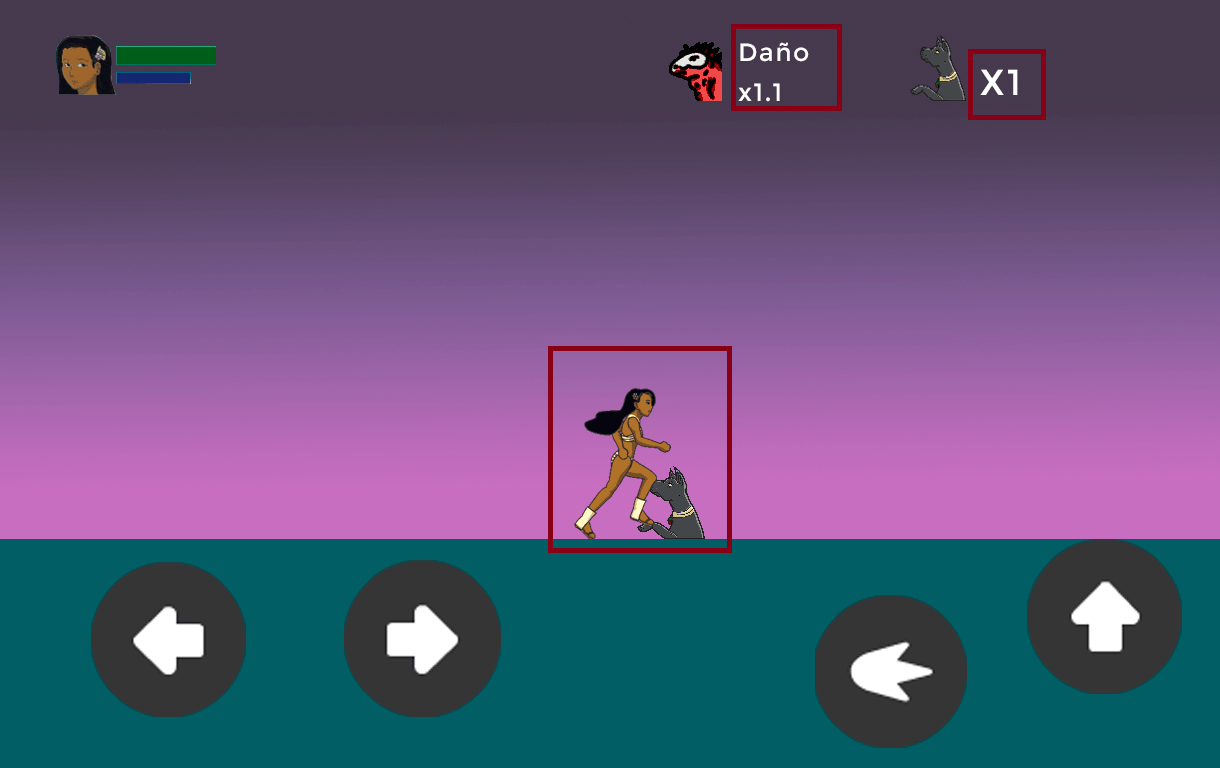
\includegraphics[width=0.4 \textwidth]{Imagenes/nivel02_xoloContacto}
  \caption{Cuando el jugador hace contacto con un Xoloitzcuintle los indicadores se modifican.}
  \label{fig:InterNivel2}
\end{figure} 

\begin{figure}
  \centering
   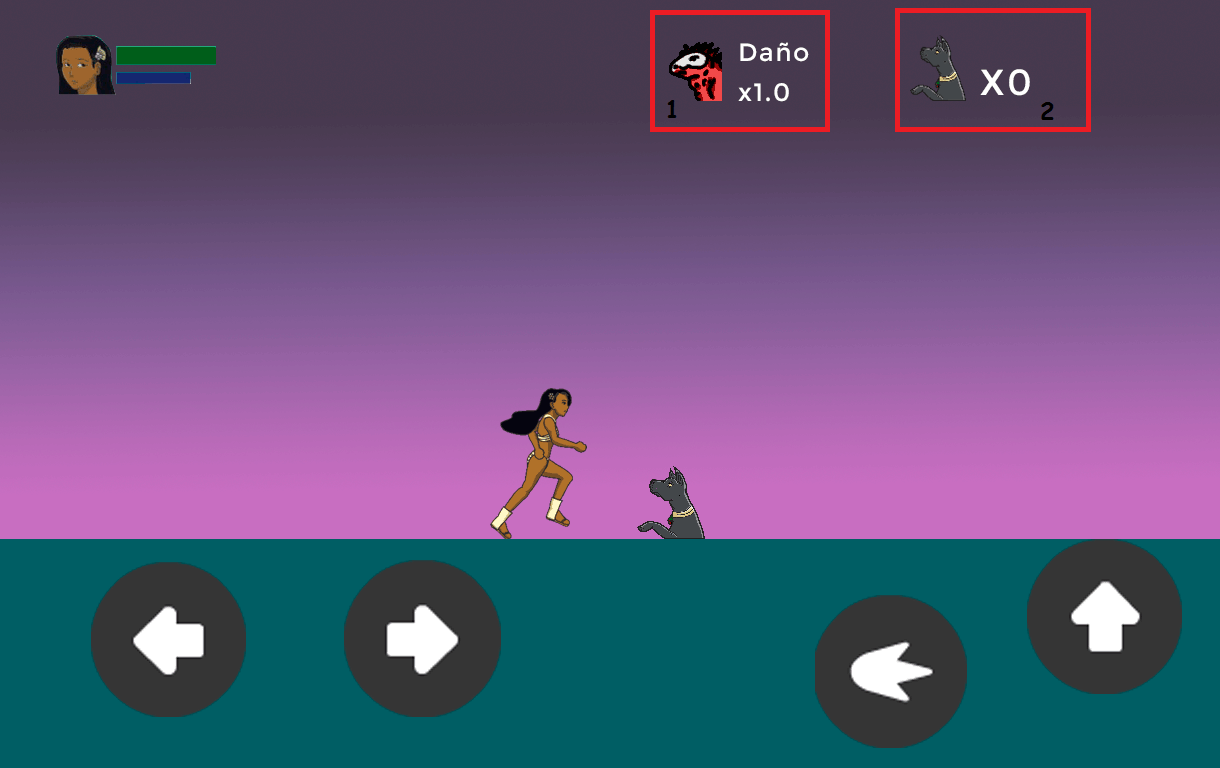
\includegraphics[width=0.4 \textwidth]{Imagenes/nivel02_xolo}
  \caption{1. Indicador de la cantidad de daño que puede efectuar Xochitonal. 2. Indicador de la cantidad de Xoloitzcuintles tocados.}
  \label{fig:GUICtrlNivel2}
\end{figure} 



	\subsection{Progreso}
Al final del nivel el jugador:
\begin{itemize}
	\item Obtendrá una mejora en la cantidad de vida de Malinalli.
	\item El jugador podrá ver las siguientes cinemáticas(Para mayor información sobre cada una, ver el guion literario del juego)
		\begin{itemize}
			\item Cinemática 6 (ver apartado \ref{Cin:Cinematica06}).
			\item Cinemática 7 (ver apartado \ref{Cin:Cinematica07}).
			\item Cinemática 8 (ver apartado \ref{Cin:Cinematica08}).
			\item Cinemática 9 (ver apartado \ref{Cin:Cinematica09}).
			\item Cinemática 10 (ver apartado \ref{Cin:Cinematica10}).
		\end{itemize}
	\item Tendrá disponible el tercer nivel del juego \ref{Nivel:Niv03} en el menú de selección de nivel (ver apartado \ref{inter:interfaz03}). 
\end{itemize}
	\subsection{Enemigos}
	\begin{itemize}
		\item Fantasma rojo (ver apartado \ref{per:fantasmaR}).
			
		\item Fantasma morado (ver apartado \ref{per:fantasmaM}).
			
		\item Piedras filosas (ver apartado \ref{obs:piedrasF}).
		\item Xochitonal (ver apartado \ref{per:xochitonal}).
			
	\end{itemize}
	\subsection{Items}
	\begin{itemize}
		\item Xoloitzcuintles (ver apartado\ref{item:Xolo}).
		\item Grano de cacao.
		\item Flor de vainilla.
	\end{itemize}
	\subsection{Personajes}
	\begin{itemize}
		\item Malinalli (ver apartado \ref{per:malinalli}).
		\item Xolotl (ver apartado \ref{per:xolotl}).
			
		\item Xochitonal (ver apartado \ref{per.xochitonal}).
	\end{itemize}
	
\subsection{Escenario}
\begin{itemize} 
	\item Fondo:
Montañas en el plano más alejado, y a sus pies una pequeña linea que muestre la orilla del río. El cielo es de color verde en degradado con negro.
	\item Suelo:
		\begin{itemize}
			\item Agua: Será utilizada durante la zona de plataformas y durante la batalla contra el jefe del nivel.
			\item Suelo con pasto: Será usado durante la cinemática 4 (ver apartado \ref{Cin:Cinematica04}) y la cinemática 8 (ver apartado \ref{Cin:Cinematica08}).
		\end{itemize}
	\item Obstáculos:
		\begin{itemize}
			\item Piedras filosas. Ver en \ref{obs.piedrasF}.				
		\end{itemize}
	\item Objetos de fondo: 
	\\
	\par	
	Sin objetos de fondo.
	
\end{itemize}	
	
	\subsection{Referencia a BGM y SFX}
\begin{itemize}
	\item BGM:
		\begin{itemize}
			\item Música plataforma segundo nivel (Ver apartado \ref{Musica:N02_ZN01})
			\item Música jefe segundo nivel (Ver apartado\ref{Musica:N02_ZN02}).
		\end{itemize}
	\item SFX:
		\begin{itemize}
			\item Explosión de agua (Ver apartado \ref{SFX:ExpAgua}).
			\item Salpicadura de agua (Ver apartado \ref{SFX:SalAgua}).
		\end{itemize}
\end{itemize}
	\subsection{Referencia a FX}
\begin{itemize}
	\item Oleaje (Ver apartado \ref{FX:Oleaje}).
	\item Salpucadura de agua (Ver apartado \ref{FX:SalAgua}).
	\item Explosión de burbuja (Ver apartado \ref{FX:ExpAgua}).
	\item Explosión de energía tonalli rojo (Ver apartado \ref{FX:ExpTonR}).
		 
\end{itemize}
